\chapter{Introducción a Arduino}
\section{\obj}
\capacidad
\begin{itemize}
    \item Desarrollar un programa sencillo en la plataforma de Arduino.
    \item Implementar en C las funciones lógicas AND, OR, XOR, NAND y NOR
\end{itemize}

\section{\mat}
\begin{itemize}
\item 1 Arduino UNO MINIMA R4.
\item 1 Multímetro.
\item 5 Resistencias de 270 o \SI{330}{\ohm}.
\item 2 Resistencias de \SI{1}{\kilo\ohm}
\item 2 interruptores pulsadores.
\item 1 Protoboard.
\item 5 Diodos emisor de luz (LEDs).
\item 2 Generadores de funciones.
\item 2 Osciloscopio.
\item 1 Computadora portátil.
\end{itemize}

\section{\pro}

Este laboratorio tiene una duración de 4 lecciones, repartidas en dos semanas. Los estudiantes deben mostrar durante las clases programadas las tres actividades propuestas. Deben recabar fotografías y resultados de los equipos de medición para elaborar las evidencias. Las evidencias se subirán al TecDigital la semana siguiente finalizadas las actividades.

\section{Práctica en Clase}

\subsection{Actividad 1}
El  código del apéndice \ref{ApendiceA1} apaga y enciende un LED según el estado de un botón. La figura \ref{fig:fig1} muestra el esquema básico de conexión.

Elimine el botón y alimente el Arduino con un generador de funciones que brinde una señal cuadrada de 0 a 5 voltios. Conecte los dos canales del osciloscopio en la  entra y salida. Recuerde que todas las tierras deben estar conectadas entre si. 

\subsubsection{Conteste las preguntas:}
¿Cuanto es el retardo de la señal?
¿Cual es la frecuencia de la señal de entrada en que la señal de salida se distorsiona? Es decir, la señal de salida no es  inversa a la señal de entrada. Recuerde capturar las pantallas del osciloscopio en ambos casos.

\begin{figure}[H]
    \tikzset{dig/.style={muxdemux, muxdemux def={Lh=5, Rh=5, NL=2, NB=0, NR=0, w=2}}}
    \centering
    \begin{circuitikz} 
        \draw 
        (0,3.5) 
        node[dig] (p){\rotatebox{90}{\small power}}
        (0,0) 
        node[dig] (m){\rotatebox{90}{\small digital IO}};
        \draw (m.blpin 1) node[above left]{\small DIO2};
        \draw (m.blpin 2) node[above left]{\small DIO4};
        \draw (p.blpin 1) node[above left]{\small 5V};
        \draw (p.blpin 2) node[above left]{\small GND};
        \coordinate (A) at (-8,2.5);
        \coordinate (B) at (-8,1);
        \coordinate (C) at (-6,2.5);
        \coordinate (D) at (-6,1);
        \coordinate (E) at (-4,2.5);
        \coordinate (F) at (-4,1);
        \coordinate (G) at (-4,0.5);
        \coordinate (H) at (-4,-1);
        \node at (-4,0.7)[jump crossing, scale = 2](X){};
        \draw[black]
        (p.blpin 1)
        -|
        (A)
        to [R, l=\SI{10}{\kilo\ohm}]
        (B)
        |-
        (X.west)
        (p.blpin 2)
        -|
        (C)
        to [push button]
        (D)
        |-
        (X.west)
        (X.east)
        --
        (m.blpin 1)
        (p.blpin 2)
        -|
        (E)
        to[led]
        (F)       
        --
        (G)     
        to [R,l=\SI{500}{\ohm}]
        (H)
        --
        ++(0,-0.5)
        --
        ++(1,0)
        |-
        (m.blpin 2)
        ;        
        \draw[dashed,blue]
        (-2.5,6) -- (1,6)node[midway, below]{ARDUINO UNO} -- (1,-1.5) -- (-2.5,-1.5) -- cycle;
    \end{circuitikz}
    \caption{Conexión de circuito para Actividad 2}
    \label{fig:fig1}
\end{figure}

\subsection{Actividad 2}

Esta actividad permite analizar el comportamiento de las conectivas lógicas  AND, OR, XOR, NAND, y NOT, y exportar los resultados al puerto serial, así como mostrar los resultados mediante los LEDs conectados a los pines $\left\lbrace4, 5, 6, 7, 8 \right\rbrace$ ; el código de ejemplo se muestra en el apéndice \ref{ApendiceA2}. 
Las entradas declaradas mediante los pines $\left\lbrace2, 3 \right\rbrace$ reciben las señales de dos generadores de funciones. 
Los generadores brindan una señal triangular que oscila ente $[0-5]$ voltios, debe ajustar cuidadosamente con el osciloscopio cada señal. 
La señal del pin 2 tendrá una frecuencia del doble del pin 3. Adicionalmente las señales  triangulares alimentaran el convertidor Analógico-Digital (ADC) mediante los pines A0 y A1. 
Conecte su Arduino según el esquema de la Figura \ref{fig:fig2}.  


\begin{figure}[H]
    \tikzset{pow/.style={muxdemux, muxdemux def={Lh=5, Rh=5, NL=2, NB=0, NR=0, w=2}}}
    \tikzset{dig/.style={muxdemux, muxdemux def={Lh=10, Rh=10, NL=7, NB=0, NR=0, w=2}}}
    \centering
    \begin{circuitikz} 
        \draw 
        (0,3.5) 
        node[pow] (p){\rotatebox{90}{\small power}}
        (0,-2) 
        node[dig] (m){\rotatebox{90}{\small digital IO}};
        \draw (m.blpin 1) node[above left]{\small DIO2};
        \draw (m.blpin 2) node[above left]{\small DIO3};
        \draw (m.blpin 3) node[above left]{\small DIO4};
        \draw (m.blpin 4) node[above left]{\small DIO5};
        \draw (m.blpin 5) node[above left]{\small DIO6};
        \draw (m.blpin 6) node[above left]{\small DIO7};
        \draw (m.blpin 7) node[above left]{\small DIO8};
        \draw (p.blpin 1) node[above left]{\small 5V};
        \draw (p.blpin 2) node[above left]{\small GND};
        \coordinate (A) at (-8,2.5);
        % \coordinate (B) at (-8,1);
        % \coordinate (C) at (-6,2.5);
        % \coordinate (D) at (-6,1);
        % \coordinate (E) at (-4,2.5);
        % \coordinate (F) at (-4,1);
        % \coordinate (G) at (-4,0.5);
        % \coordinate (H) at (-4,-1);
        % \node at (-4,0.7)[jump crossing, scale = 2](X){};
        \draw[black]
        (p.blpin 1)
        -|
        (A)
        % to [R, l=\SI{10}{\kilo\ohm}]
        % (B)
        % |-
        % (X.west)
        % (p.blpin 2)
        % -|
        % (C)
        % to [push button]
        % (D)
        % |-
        % (X.west)
        % (X.east)
        % --
        % (m.blpin 1)
        % (p.blpin 2)
        % -|
        % (E)
        % to[led]
        % (F)       
        % --
        % (G)     
        % to [R,l=\SI{500}{\ohm}]
        % (H)
        % --
        % ++(0,-0.5)
        % --
        % ++(1,0)
        % |-
        % (m.blpin 2)
        ;        
        \draw[dashed,blue]
        (-2.5,6) -- (1,6)node[midway, below]{ARDUINO UNO} -- (1,-1.5) -- (-2.5,-1.5) -- cycle;
    \end{circuitikz}
    \caption{Conexión de circuito para Actividad 3}
    \label{fig:fig3}
\end{figure}

\begin{figure}[H]
	\centering
	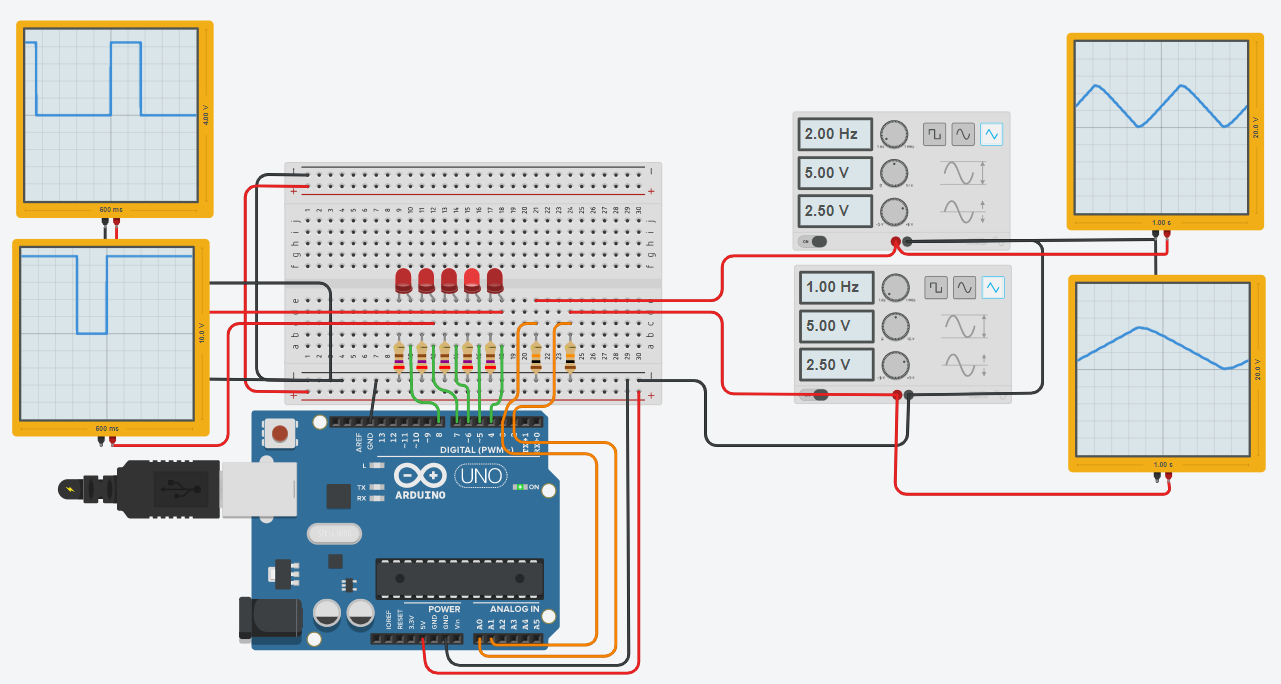
\includegraphics[width=0.8\linewidth]{Fig2.png}
	\caption{Esquema de conexión del Arduino, Generador de funciones y Osciloscopio}
	\label{fig:fig2}
\end{figure}


El código del Anexo B implementa las funciones lógicas AND, OR. Un repaso de como implementar funciones en C se muestra en \href{https://aprendiendoarduino.wordpress.com/2016/11/16/funciones-definidas-por-usuario-2/}{este enlace.} 

\subsubsection{Conteste las preguntas:}

Guarde los datos del puerto serial en un archivo .TXT e importelos en MS EXCEL para graficar los datos.
Se recomienda utilizar el monitor serial de MS CODE STUDIO dado que este permite salvar los datos.
¿Se logra apreciar las señales triangulares y digitales?
¿Las gráficas de las señales digitales de entrada y salida cumplen las tablas de verdad de las conectivas lógicas?
¿Cual es el voltaje de entrada en bajo máximo $V_{IL} max$?,
¿Cual es el voltaje de entrada en alto mínimo $V_{IH} min$?,
¿Cual es el error que presenta las mediciones de los voltajes ?,
¿Si desea un error de $\pm1$ mV, de cuantos bits debe ser el ADC?¿Explique?